\def\year{2017}\relax
%File: formatting-instruction.tex
\documentclass[letterpaper]{article} %DO NOT CHANGE THIS
\usepackage{aaai17}  %Required
\usepackage{times}  %Required
\usepackage{helvet}  %Required
\usepackage{courier}  %Required
\usepackage{url}  %Required
\usepackage{graphicx}  %Required
\frenchspacing  %Required
\setlength{\pdfpagewidth}{8.5in}  %Required
\setlength{\pdfpageheight}{11in}  %Required
\usepackage{algorithm}
\usepackage{algorithmic}
\usepackage{amssymb}
\usepackage{graphicx}
\graphicspath{ {images/} }
%PDF Info Is Required:
  \pdfinfo{
/Title (Edge Grasp Classification in Deep Learning)
/Author (Dian Wang)}
\setcounter{secnumdepth}{0}  
 \begin{document}
% The file aaai.sty is the style file for AAAI Press 
% proceedings, working notes, and technical reports.
%

\title{Edge Grasp Classification in Deep Learning}
\author{Dian Wang\\
Northeastern University, Boston, MA\\
{wang.dian@husky.neu.edu}
}
\maketitle
\begin{abstract}
This paper considers the problem of the influence of table edge or shelf edge to grasp pose detection in point clouds. A model is trained to take point cloud and grasp configurations as input to classify each grasp as either edge grasp that is pointing to an edge of table or shelf, or a non-edge grasp that is pointing to an actual object. This paper benchmark two representation of potential grasp, and two convolutional neural networks is built corresponding to the two representations. Experiments were performed to compare those two methods. The analysis shows…
\end{abstract}

\section{Introduction}
\noindent Grasping is one of the most intuitive and the most widely applied technology in robotics. Recently, researchers have proposed grasp detection methods that estimate potential grasps independently of object identity. Those methods take RGBD image or point cloud from depth sensor as input and generate output of various grasp configurations. 

Those methods are promising and reliable. \cite{RN6} achieved a 93\% end-to-end grasp success rate for novel objects presented in dense clutter with their grasp pose detection (GPD) method. However, one problem of such method is that in practical grasping applications which aim to grasp object on table or shelf, some grasp pointing to the edge of table or shelf may be regarded as good grasp. 

In this paper, a series of methods are proposed that make GPD avoid that problem. First, 2 grasp representation methods are used to turn raw data from point cloud as well as grasp configuration into image that can be used for neural network input. Second, 2 convolutional neural networks are built respectively for those 2 representations. They take the representation image as input and output the probability for that grasp being edge grasp or non-edge grasp. Third, experiments are made to evaluate the performance of the 2 models.

\section{Background}
\noindent Grasping involves observing the environment as well as generating potential grasps from observed information. Some grasp detection method like the ROS grasp pipeline \cite{RN5} build a CAD model of the target object, then calculate a trajectory that grasp the localized object. However, this approach assume that an accurate CAD model could be built for every grasping object. In contrast, GPD \cite{RN6} detect potential grasps by analyzing the local geometry and/or graspable surface.

\begin{algorithm}
\caption{Grasp Pose Detection}
\textbf{Input:} a view point cloud,  $\mathbb{C}$; a region of interest, $R$; a hand, $\Theta$; a positive integer, $\mathbb{N}$ \\
\textbf{Output:} a set of 6-DOF grasp candidates, $H\subset R$ \\
\begin{algorithmic}[1]
\STATE $\mathbb{C}'={\rm PreprocessCloud}(\mathbb{C})$
\STATE $R={\rm GetROI}(\mathbb{C}')$
\STATE $S={\rm Sample}(\mathbb{C}',R,\Theta, \mathbb{N})$
\STATE $I={\rm Encode}(S,\mathbb{C}', R, \Theta)$
\STATE $H={\rm Score}(I)$
\STATE $g={\rm SelectGrasp}(S, H)$
\end{algorithmic}  
\end{algorithm}  

Their algorithm, as is shown in Algorithm 1, works as follow. Step 1 preprocess the original point cloud. Step 2 characterize the region of interest (ROI), which is the region of the target location. Step 3 samples a series of grasp candidates from ROI. Step 4 encodes each grasp candidate as a multi-channel image. Step 5 assign each candidate a score. Those scores indicate how likely that candidate is a grasp. Step 6 select a number of grasps based on the score from step 5.

\section{Related Work}
\subsection{Choosing Grasp Heuristically}
By manually confine grasp configuration based on the known knowledge of the environment, edge grasps could be avoided. For example, a “top grasp” \cite{RN8}, which means the gripper approach-es the object from the top down, is always a non-edge grasp since the edge is always perpendicular to the gravity vector. However, this requires enough space above the grasp position. If there is only “side grasps”, the problem still exists.

\subsection{Multi-view Representation of Point Cloud}
One approach to apply machine learning methods to point cloud is using multiple views. Multi-view CNN \cite{RN7} takes 2D images from 12 different views from a 3D shape model as input, outputs object class predictions.
Based on multi-view CNN, GPD used 15 channels image representation for each grasp \cite{RN6}. For each of the x, y, and z axis, they have an averaged height map of the occupied points, an averaged height map of the unobserved region, and 3 averaged surface normal images.

\subsection{Occupancy Grid Representation of Point Cloud}
3D convolutional neural networks are also used when applying machine learning methods to point cloud data. VoxNet \cite{RN4} provided a basic 3D CNN architecture that can be applied to create fast and accurate object class detectors for point cloud data. Their method takes point cloud as input, generate occupancy grid based on that point cloud, and uses a 2-layer 3D CNN for classification.

\section{Project Description}
\subsection{Overview of Edge Grasp Classification Algorithm}
Given a point cloud and a transformation matrix representing a grasp, the edge grasp classification problem is to compute the probability of that grasp being an edge grasp or a non-edge grasp.

\begin{algorithm}[H]
\caption{Edge Grasp Classification}
\textbf{Input:} a point cloud, $\mathbb{C}$; a grasp transformation matrix, ${^h}T_b$ \\
\textbf{Output:} a probability of that grasp being edge grasp, $P\in [0, 1]$ \\
\begin{algorithmic}[1]
\STATE $I={\rm GraspRepresentation}(\mathbb{C}, {^h}T_b)$
\STATE $P={\rm Probability}(I)$
\end{algorithmic}
\end{algorithm}

My algorithm follows the steps shown in Algorithm 2. Step 1 encodes the grasp candidate into a multi-channel image from the original point cloud and the transformation matrix (from base frame to hand frame) of that grasp. Step 2 generate the probability of that grasp being an edge grasp using convolutional neural networks.

\subsection{Grasp Representation}
Each grasp candidate is represented in an image of fixed size so that it could be used for the input of convolutional neural network. The image should contain the information of the geometry of the observed grasping surface. Let $\mathbb{C}$ be the observed point cloud in base frame, and ${}^hT_b$ be the transformation matrix of a grasp from base frame to hand frame, then the point cloud in hand frame ${}^h\mathbb{C}$ is:
\begin{equation}
    {}^h\mathbb{C}={}^hT_b\mathbb{C}
\end{equation}
and the points that will be computed into image is:
\begin{equation}
    X=\{\forall {\rm point}\in {}^h\mathbb{C}|{\rm point}\in {\rm ROI}\}
\end{equation}
where ROI is the cubic region of interest.

\subsubsection{Multiple View Representation.}
Inspired by the representation in GPD \cite{RN6}, this paper firstly use a 3-channel multi-view image. Specifically, $X$ is projected onto 3 planes orthogonal to the 3 axes of the hand frame. For example, the projection of the (x, y) plane is calculated as follows:
For point $X[i]$, its (x, y) coordinates $C(x, y)[i]$ in the projection image is computed as:
\begin{equation}
    C(x, y)[i]=\frac{p-1}{l} (X(x, y)[i] + \frac {l} 2)
\end{equation}
where $X(x, y)[i]$ is the x, y value of point $X[i]$, p is the number of the pixels in the square projection image, and l is the length of the cubic ROI. $C(x, y)[i]\in [0, p)$ and $C(x, y)[i]\in \mathbb{N}$

The value $V(x, y)[i]$ of point $X[i]$ in the projection image is computed as:
\begin{equation}
    V(x, y)[i]=\frac{X(z)[i]+\frac{l}{2}}{l}
\end{equation}
where $X(z)[i]$ is the z value of point $X[i]$. $V(x, y)[i]\in [0, 1]$. After the coordinates and values of each point is computed, the image $I(x, y)$ is computed as:

\begin{algorithm}[H]
\caption{Projection Image for (x, y) Plane}
\textbf{Input:} coordinates $C=C(x, y)$; values $V=V(x, y)$\\
\textbf{Output:} projection image in (x, y) plane, $I=I(x,y)$ \\
\begin{algorithmic}[1]
\FOR {$i = 0 \to p-1$}
\FOR {$j = 0 \to p-1$} 
\STATE $I[i, j] = 0$
\ENDFOR
\ENDFOR
\FOR {$i = 0 \to n$}
\STATE $I[C[i].x, C[i].y]=\max(I[C[i].x, C[i].y], V[i])$
\ENDFOR
\STATE $I={\rm GrayDilation}(I)$
\end{algorithmic}
\end{algorithm}

The value of a particular pixel in the image is the max value of all points that is assigned into the coordinate of that pixel. Gray dilation \cite{BK1} is applied to avoid the influence of void pixels.

After applying above methods to 3 planes orthogonal to the 3 axis of the hand reference frame, a $3\times p \times p$ image is generated for a grasp candidate.

\subsubsection{3D Occupancy Grid Representation.} This paper also use a 3 dimensional occupancy grid image, where $X$ is transformed into a binary 3D image. The 3D image is calculated as follows:
For point $X[i]$, its coordinates $C'[i]$ in the occupancy image is computed as:
\begin{equation}
    C'[i]=\frac{p-1}{l} (X[i]+\frac{l}{2}
\end{equation}
where $C'[i]\in [0, p)$ and $C'[i]\in \mathbb{N}$. The image $I'$ is computed as:
\begin{algorithm}[H]
\caption{Occupancy Image}
\textbf{Input:} coordinates $C'$\\
\textbf{Output:} occupancy image, $I'$\\
\begin{algorithmic}[1]
\FOR {$i = 0 \to p-1$}
\FOR {$j = 0 \to p-1$}
\FOR {$k = 0 \to p-1$}
\STATE $I[i, j, k] = 0$
\ENDFOR
\ENDFOR
\ENDFOR
\FOR {$i = 0 \to n$}
\STATE $I[C[i].x, C[i].y, C[i].z]=1$
\ENDFOR
\STATE $I={\rm BinaryDilation}(I)$
\end{algorithmic}
\end{algorithm}

The value of a particular pixel in the image is 1 if at least 1 point is assigned into the coordinate of that pixel, or the value will be 0. Similarly, binary dilation \cite{BK1} is applied to avoid the influence of void pixels.

After applying above methods, a $p\times p\times p$ image is generated for a grasp candidate.

\subsection{Convolutional Neural Networks}
Convolutional neural networks are applied to computing the probability. This paper use PyTorch \cite{Pytorch} to implement CNNs.

\subsubsection{2.5D CNN for Projection Image.} This paper used the basic structure of LeNet\cite{RN3}. The detailed structure is:
\begin{figure}[H]
    \centering
    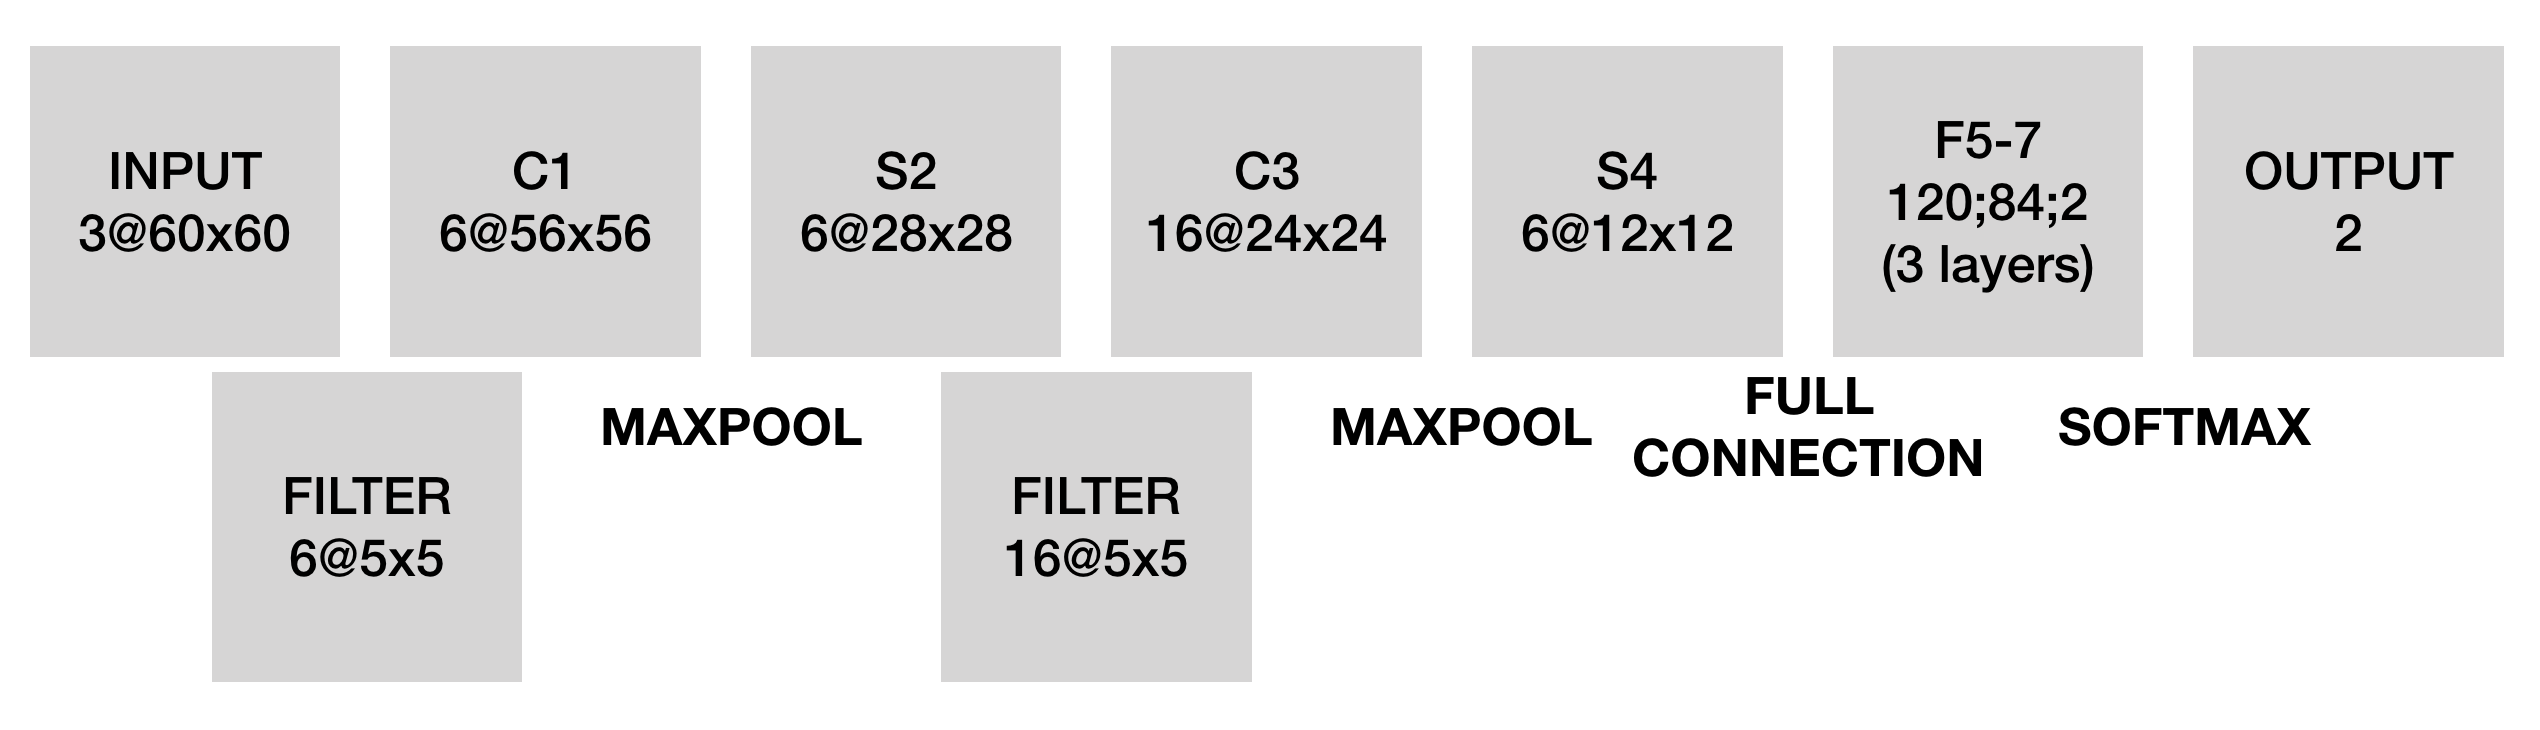
\includegraphics[width=8cm]{images/CNN.png}
    \caption{Structure of CNN}
    \label{fig:my_label}
\end{figure}
The input is $3\times60\times60$ projection image from above multiple view representation. A $6\times5\times5$ filter is applied first, which produce a $6\times56\times56$ hidden layer. The second filter with size $16\times5\times5$ is applied after max pooling, then max pooling again. After that, 3 full connection layer is used, and Softmax function generate the output. The output of this CNN is 2 probabilities, representing the input grasp image being edge grasp and non-edge grasp.

\subsubsection{3D CNN for Occupancy Image.} This paper further applied a 3 dimensional convoluntional neural network to the occupancy grid image. The structure is inspired by VoxNet \cite{RN4}. 



\clearpage
\section{Formatting Requirements in Brief}
We need source and PDF files that can be used in a variety of ways and can be output on a variety of devices. The design and appearance of the paper is governed by the aaai style file. You must not make any changes to this file, nor use any commands, packages, style files, or macros that alter that design, including, but not limited to spacing, floats, margins, fonts, font size, and appearance. AAAI imposes  requirements on your source and PDF files that must be followed. Most of these requirements are based on our efforts to standardize conference manuscript properties and layout. All papers submitted to AAAI for publication must comply with the following:

\begin{itemize}
\item Your .tex file must compile in PDF\LaTeX{} --- \textbf{ no .ps or .eps figure files.}
\item All fonts must be embedded in the PDF file --- \textbf{ this includes your figures.}
\item Modifications to the style file, whether directly or via commands in your document may not be made, most especially when made in an effor to avoid extra page charges or make your paper fit in a specific number of pages.
\item No type 3 fonts may be used (even in illustrations).
\item You may not alter the spacing above and below captions, figures, headings, and subheadings.
\item You may not alter the font sizes of text elements, footnotes, heading elements, captions, or title information (for references and tables and mathematics, please see the the limited exceptions provided herein).
\item You may not alter the line spacing of text.
\item Your title must follow Title Case capitalization rules (not sentence case).
\item Your .tex file include completed metadata to pass-through to the PDF (see PDFINFO below)
\item \LaTeX{} documents must use the Times or Nimbus font package (do not use Computer Modern for the text of your paper).
\item No \LaTeX{} 209 documents may be used or submitted.
\item Your source must not require use of fonts for non-Roman alphabets within the text itself. If your paper includes symbols in other languages (such as, but not limited to Arabic, Chinese, Hebrew, Japanese, Russian and other Cyrillic languages), you must restrict their use to figures.
\item Fonts that require non-English language support (CID and Identity-H) must be converted to outlines or 300 dpi bitmap or removed from the document (even if they are in a graphics file embedded in the document). 
\item Two-column format in AAAI style is required for all papers.
\item The paper size for final submission must be US letter without exception.
\item The source file must exactly match the PDF.
\item The document margins must be as specified in the formatting instructions.
\item The number of pages and the file size must be as specified for your event.
\item No document may be password protected.
\item Neither the PDFs nor the source may contain any embedded links or bookmarks.
\item Your source and PDF must not have any page numbers, footers, or headers.
\item Your PDF must be compatible with Acrobat 5 or higher.
\item Your \LaTeX{} source file (excluding references) must consist of a \textbf{single} file (use of the ``input" command is not allowed.
\item Your graphics must be sized appropriately outside of \LaTeX{} (do not use the ``clip" command) .
\end{itemize}

If you do not follow the above requirements, it is likely that we will be unable to publish your paper.

\section{What Files to Submit}
You must submit the following items to ensure that your paper is published:
\begin{itemize}
\item A fully-compliant PDF file.
\item Your  \LaTeX{}  source file submitted as a \textbf{single} .tex file (do not use the ``input" command to include sections of your paper --- every section must be in the single source file). The only exception is the reference list, which you should include separately. Your source must compile on our system, which includes the standard \LaTeX{} support files.
\item Only the graphics files used in compiling paper.
\item The \LaTeX{}-generated files (e.g. .aux and .bib file, etc.) for your compiled source.
\item If you have used an old installation of \LaTeX{}, you should include algorithm style files). If in doubt, include it.
\end{itemize}

Your \LaTeX{} source will be reviewed and recompiled on our system (if it does not compile, you may incur late fees).   \textbf{Do not submit your source in multiple text files.} Your single \LaTeX{} source file must include all your text, your bibliography (formatted using aaai.bst), and any custom macros. Accompanying this source file, you must also supply any nonstandard (or older) referenced style files and all your referenced graphics files. 

Your files should work without any supporting files (other than the program itself) on any computer with a standard \LaTeX{} distribution. Place your PDF and source files in a single tar, zipped, gzipped, stuffed, or compressed archive. Name your source file with your last (family) name.

\textbf{Do not send files that are not actually used in the paper.} We don't want you to send us any files not needed for compiling your paper, including, for example, this instructions file, unused graphics files, standard style files, and so forth.

\textbf{Obsolete style files.}  The commands for some common packages (such as some used for algorithms), may have changed. Please be certain that you are not compiling your paper using old or obsolete style files. 

\section{Using \LaTeX{} to Format Your Paper}

The latest version of the AAAI style file is available on AAAI's website. Download this file and place it in  the \TeX\ search path. Placing it in the same directory as the paper should also work. You must download the latest version of the complete author kit so that you will have the latest instruction set and style file.

\subsection{Document Preamble}

In the \LaTeX{} source for your paper, you \textbf{must} place the following lines as shown in the example in this subsection. This command set-up is for three authors. Add or subtract author and address lines as necessary, and uncomment the portions that apply to you. In most instances, this is all you need to do to format your paper in the Times font. The helvet package will cause Helvetica to be used for sans serif. These files are part of the PSNFSS2e package, which is freely available from many Internet sites (and is often part of a standard installation).

Leave the setcounter for section number depth commented out and set at 0 unless you want to add section numbers to your paper. If you do add section numbers, you must uncomment this line and change the number to 1 (for section numbers), or 2 (for section and subsection numbers). The style file will not work properly with numbering of subsubsections, so do not use a number higher than 2.

If (and only if) your author title information will not fit within the specified  height allowed, put \textbackslash setlength \textbackslash titlebox{2.5in} in your preamble. Increase the height until the height error disappears from your log. You may not use the  \textbackslash setlength command elsewhere in your paper, and it may not be used to reduce the height of the author-title box.

\subsubsection{The Following Must Appear in Your Preamble}
\begin{quote}
\begin{scriptsize}\begin{verbatim}
\documentclass[letterpaper]{article}
\usepackage{aaai}
\usepackage{times}
\usepackage{helvet}
\usepackage{courier}
\usepackage{url}
\usepackage{graphicx}
\frenchspacing
% Add additional packages here. The following
% packages may NOT be used  (this list
% is not exhaustive:
% authblk, caption, CJK, float, fullpage, geometry, 
%hyperref, layout, nameref, natbib, savetrees, 
%setspace, titlesec, tocbibind, ulem
%
%US Lettersize Paper Is Required
\setlength{pdfpagewidth}{8.5in}
\setlength{pdfpageheight}{11in}\\
%
%
% PDFINFO
% You are required to complete the following
% for pass-through to the PDF. 
% No LaTeX commands of any kind may be
% entered. The parentheses and spaces 
% are an integral part of the 
% pdfinfo script and must not be removed.
%
\pdfinfo{
/Title (Input Your Paper Title Here)
/Author (John Doe, Jane Doe)
/Keywords (Input your keywords in this optional area)
}
%
%Section Numbers
% Uncomment if you want to use section numbers
% and change the 0 to a 1 or 2
% \setcounter{secnumdepth}{0}

% Title and Author Information Must Immediate Follow
% the pdfinfo within the preamble
%
\title{Title}\\
\author\{Author 1 \ and Author 2\\
Address line\\
Address line\\
\ And\\
Author 3\\
Address line\\
Address line
}\\
%
\end{verbatim}\end{scriptsize}
\end{quote}

\subsection{Preparing Your Paper}

After the preamble above, you should prepare your paper as follows:
\begin{quote}
\begin{scriptsize}\begin{verbatim}
%
\begin{document}
\maketitle
\begin{abstract}
%...
\end{abstract}\end{verbatim}\end{scriptsize}
\end{quote}

\subsubsection{The Following Must Conclude Your Document}
\begin{quote}
\begin{scriptsize}\begin{verbatim}
%References and End of Paper
%These lines must be placed at the end of your paper
\bibliography{Bibliography-File}
\bibliographystyle{aaai}
\end{document}
\end{verbatim}\end{scriptsize}
\end{quote}

\subsection{Inserting Document Metadata with \LaTeX{}}
PDF files contain document summary information that enables us to create an Acrobat index (pdx) file, and also allows search engines to locate and present your paper more accurately. \textit{Document metadata  for author and title are REQUIRED.} 

\textit{Important:} Do not include \textit{any} \LaTeX{} code or nonascii characters (including accented characters) in the metadata. The data in the metadata must be completely plain ascii. It may not include slashes, accents, linebreaks, unicode, or any \LaTeX{} commands. Type the title exactly as it appears on the paper (minus all formatting). Input the author names in the order in which they appear on the paper (minus all accents), separating each author by a comma. You may also include keywords in the Keywords field.




\begin{quote}
\begin{small}
\textbackslash begin\{document\}\\
\textbackslash maketitle\\
...\\
\textbackslash bibliography\{Bibliography-File\}\\
\textbackslash bibliographystyle\{aaai\}\\
\textbackslash end\{document\}\\
\end{small}
\end{quote}
\subsection{Incompatible Packages}
The following packages are incompatible with aaai.sty and/or aaai.bst and must not be used (this list is not exhaustive --- there are others as well):
\begin{itemize}
\item authblk
\item caption 
\item CJK
\item float
\item fullpage
\item geometry
\item hyperref
\item layout
\item nameref
\item natbib
\item savetrees
\item setspace
\item titlesec
\item tocbibind
\item ulem
\item T1 fontenc package (install the CM super fonts package instead)
\end{itemize}


\subsection{Illegal Commands}
The following commands may not be used in your paper (this list is not exhaustive --- there are others; generally, if it alters floats, margins, fonts, linespacing, or the presentation of the references and citations, it is unacceptable:
\begin{itemize}
\item \textbackslash renewcommand (in almost all instances)
\item baselinestretch
\item \textbackslash setlength (except for titlebox)
\item \textbackslash input
\item \textbackslash vspace or vskip (when used before or after a section or subsection)
\item \textbackslash addtolength 
\item \textbackslash columnsep
\item \textbackslash top margin (or text height or addsidemargin or even side margin)
\item trim or clip (used to crop figures)
\item any command that globally alters floats, space above and below figures and tables
\end{itemize}

\subsection{Illegal Commands in Final Paper}
For your final camera ready copy, you must not use any page break commands, including, but not limited to:
\begin{itemize}
\item \textbackslash newpage
\item \textbackslash break
\item \textbackslash clearpage
\item \textbackslash pagebreak
\end{itemize}
(References must flow directly after the text without breaks.) Note that this may \textit{not} the case when submitting a paper for review. Some conferences require references to be on a separate page during the review process. AAAI Press, however, does not require this condition for the final paper.


\subsection{Paper Size, Margins, and Column Width}
Papers must be formatted to print in two-column format on 8.5 x 11 inch US letter-sized paper. The margins must be exactly as follows: 
\begin{itemize}
\item Top margin: .75 inches
\item Left margin: .75 inches
\item Right margin: .75 inches
\item Bottom margin: 1.25 inches
\end{itemize} 


The default paper size in most installations of \LaTeX{} is A4. However, because we require that your electronic paper be formatted in US letter size, you will need to alter the default for this paper to US letter size. Assuming you are using the 2e version of \LaTeX{}, you can do this by including the [letterpaper] option at the beginning of your file: 
\textbackslash documentclass[letterpaper]{article}. 

This command is usually sufficient to change the format. Sometimes, however, it may not work. Use PDF\LaTeX{} and include
\textbackslash setlength\{\textbackslash pdfpagewidth\}\{8.5in\}
\textbackslash setlength\{\textbackslash pdfpageheight\}\{11in\}
in your preamble. 

\textbf{Do not use the Geometry package to alter the page size.} Use of this style file alters aaai.sty and will result in your paper being rejected. 


\subsubsection{Column Width and Margins.}
To ensure maximum readability, your paper must include two columns. Each column should be 3.3 inches wide (slightly more than 3.25 inches), with a .375 inch (.952 cm) gutter of white space between the two columns. The aaai.sty file will automatically create these columns for you. 

\subsection{Overlength Papers}
If your paper is too long, turn on \textbackslash frenchspacing, which will reduce the space after periods. Next,  shrink the size of your graphics. Use \textbackslash centering instead of \textbackslash begin\{center\} in your figure environment. For mathematical environments, you may reduce fontsize. You may also alter the size of your bibliography by inserting \textbackslash fontsize\{9.5pt\}\{10.5pt\} \textbackslash selectfont
right before the bibliography (the minimum size is \textbackslash fontsize\{9.0pt\}\{10.0pt\}. 

Commands that alter page layout are forbidden. These include \textbackslash columnsep, \textbackslash topmargin, \textbackslash topskip, \textbackslash textheight, \textbackslash textwidth, \textbackslash oddsidemargin, and \textbackslash evensizemargin (this list is not exhaustive). If you alter page layout, you will be required to pay the page fee \textit{plus} a reformatting fee. Other commands that are questionable and may cause your paper to be rejected include  \textbackslash parindent, and \textbackslash parskip. Commands that alter the space between sections are forbidden. The title sec package is not allowed. Regardless of the above, if your paper is obviously ``squeezed" it is not going to to be accepted. Before using every trick you know to make your paper a certain length, try reducing the size of your graphics or cutting text instead or (if allowed) paying the extra page charge.

\subsection{Figures}
Your paper must compile in PDF\LaTeX{}. Consequently, all your figures must be .jpg, .png, or .pdf. You may not use  the .gif (the resolution is too low), .ps, or .eps file format for your figures.

When you include your figures, you must crop them \textbf{outside} of \LaTeX{}. The command \textbackslash includegraphics*[clip=true, viewport 0 0 10 10]{...} might result in a PDF that looks great, but the image is \textbf{not really cropped.} The full image can reappear (and obscure whatever it is overlapping) when page numbers are applied or color space is standardized. 

\subsection{Type Font and Size}
Your paper must be formatted in Times Roman or Nimbus. We will not accept papers formatted using Computer Modern or Palatino or some other font as the text or heading typeface. Sans serif, when used, should be Courier. Use Symbol or Lucida or Computer Modern for \textit{mathematics only. } 

Do not use type 3 fonts for any portion of your paper, including graphics. Type 3 bitmapped fonts are designed for fixed resolution printers. Most print at 300 dpi even if the printer resolution is 1200 dpi or higher. They also often cause high resolution imagesetter devices and our PDF indexing software to crash. Consequently, AAAI will not accept electronic files containing obsolete type 3 fonts. Files containing those fonts (even in graphics) will be rejected. 

Fortunately, there are effective workarounds that will prevent your file from embedding type 3 bitmapped fonts. The easiest workaround is to use the required times, helvet, and courier packages with \LaTeX{}2e. (Note that papers formatted in this way will still use Computer Modern for the mathematics. To make the math look good, you'll either have to use Symbol or Lucida, or you will need to install type 1 Computer Modern fonts --- for more on these fonts, see the section ``Obtaining Type 1 Computer Modern.")

If you are unsure if your paper contains type 3 fonts, view the PDF in Acrobat Reader. The Properties/Fonts window will display the font name, font type, and encoding properties of all the fonts in the document. If you are unsure if your graphics contain type 3 fonts (and they are PostScript or encapsulated PostScript documents), create PDF versions of them, and consult the properties window in Acrobat Reader. 

The default size for your type should be ten-point with twelve-point leading (line spacing). Start all pages (except the first) directly under the top margin. (See the next section for instructions on formatting the title page.) Indent ten points when beginning a new paragraph, unless the paragraph begins directly below a heading or subheading.

\subsubsection{Obtaining Type 1 Computer Modern for \LaTeX{}.}

If you use Computer Modern for the mathematics in your paper (you cannot use it for the text) you may need to download type 1 Computer fonts. They are available without charge from the American Mathematical Society:
http://www.ams.org/tex/type1-fonts.html. 

\subsection{Title and Authors}
Your title must appear in mixed case (nouns, pronouns, and verbs are capitalized) near the top of the first page, centered over both columns in sixteen-point bold type (twenty-four point leading). This style is called ``mixed case." Author's names should appear below the title of the paper, centered in twelve-point type (with fifteen point leading), along with affiliation(s) and complete address(es) (including electronic mail address if available) in nine-point roman type (the twelve point leading). (If the title is long, or you have many authors, you may reduce the specified point sizes by up to two points.) You should begin the two-column format when you come to the abstract. 

\subsubsection{Formatting Author Information}
Author information can be set in a number of different styles, depending on the number of authors and the number of affiliations you need to display. For several authors from the same institution, use \textbackslash and:

\begin{quote}\begin{scriptsize}\begin{verbatim}
\author{Author 1 \and ... \and Author n\\ 
Address line \\ ... \\ Address line}
\end{verbatim}\end{scriptsize}\end{quote}

\noindent If the names do not fit well on one line use:

\begin{quote}\begin{scriptsize}\begin{verbatim}
\author{Author 1} ... \\
{\bf \Large Author  ...  Author}\\ 
Address line \\ ... \\ Address line
}
\end{verbatim}\end{scriptsize}\end{quote}

\noindent For authors from different institutions, use \textbackslash And:

\begin{quote}\begin{scriptsize}\begin{verbatim}
\author{Author 1\\ Address line \\ ... \\ Address line 
\And ... \And Author n\\
Address line\\ ... \\ Address line}
\end{verbatim}\end{scriptsize}\end{quote}

\noindent To start a separate ``row" of authors, use \textbackslash AND:

\noindent If the title and author information does not fit in the area allocated, place
\textbackslash setlength\textbackslash titlebox\{\textit{height}\}
after the \textbackslash documentclass line where \{\textit{height}\} is  2.5in or greater.

\subsubsection{Formatting Author Information --- Alternative Method}
If your paper has a large number of authors from different institutions, you may use the following alternative method for displaying the author information.

\begin{quote}\begin{scriptsize}\begin{verbatim}
\author{AuthorOne},\textsuperscript{1}
\author{AuthorTwo},\textsuperscript{2}
\author{AuthorThree},\textsuperscript{3}
\author{AuthorFour},\textsuperscript{4}
\author{AuthorFive}, \textsuperscript{5}\\
\textsuperscript{1}AffiliationOne}\\
\textsuperscript{2}AffiliationTwo}\\
\textsuperscript{3}AffiliationThree}\\
\textsuperscript{4}AffiliationFour}\\
\textsuperscript{5}AffiliationFive}\\
\{email, email\}@affiliation.com,
email@affiliation.com,
email@affiliation.com, 
email@affiliation.com
\end{verbatim}\end{scriptsize}\end{quote}


\subsection{\LaTeX{} Copyright Notice}
The copyright notice automatically appears if you use aaai.sty. If you are creating a technical report, it is not necessary to include this notice. You may disable the copyright line using the \verb+\+nocopyrightcommand. To change the entire text of the copyright slug, use:
\textbackslash copyrighttext \{\emph{text}\}.
Either of these must appear before \textbackslash maketitle. Please be advised, however, that \textit{if you disable or change the copyright line and transfer of copyright is required, your paper will not be published.}

\subsection{Credits}
Any credits to a sponsoring agency should appear in the acknowledgments section, unless the agency requires different placement. If it is necessary to include this information on the front page, use
\textbackslash thanks in either the \textbackslash author or \textbackslash title commands.
For example:
\begin{quote}
\begin{small}
\textbackslash title\{Very Important Results in AI\textbackslash thanks\{This work is
 supported by everybody.\}\}
\end{small}
\end{quote}
Multiple \textbackslash thanks commands can be given. Each will result in a separate footnote indication in the author or title with the corresponding text at the botton of the first column of the document. Note that the \textbackslash thanks command is fragile. You will need to use \textbackslash protect.

Please do not include \textbackslash pubnote commands in your document.

\subsection{Abstract}
Follow the example commands in this document for creation of your abstract. Further indentation is not required. {Do not include references in your abstract!}

\subsection{Page Numbers}

Do not \textbf{ever} print any page numbers on your paper. 

\subsection{Text }
The main body of the paper must be formatted in ten-point with twelve-point leading (line spacing).

\subsection{Citations}
Citations within the text should include the author's last name and year, for example (Newell 1980). Append lower-case letters to the year in cases of ambiguity. Multiple authors should be treated as follows: (Feigenbaum and Engelmore 1988) or (Ford, Hayes, and Glymour 1992). In the case of four or more authors, list only the first author, followed by et al. (Ford et al. 1997).

\subsection{Extracts}
Long quotations and extracts should be indented ten points from the left and right margins. 

\begin{quote}
This is an example of an extract or quotation. Note the indent on both sides. Quotation marks are not necessary if you offset the text in a block like this, and properly identify and cite the quotation in the text. 

\end{quote}

\subsection{Footnotes}
Avoid footnotes as much as possible; they interrupt the reading of the text. When essential, they should be consecutively numbered throughout with superscript Arabic numbers. Footnotes should appear at the bottom of the page, separated from the text by a blank line space and a thin, half-point rule. 

\subsection{Headings and Sections}
When necessary, headings should be used to separate major sections of your paper. Remember, you are writing a short paper, not a lengthy book! An overabundance of headings will tend to make your paper look more like an outline than a paper. The aaai.sty package will create headings for you. Do not alter their size nor their spacing above or below. 

\subsubsection{Section Numbers}
The use of section numbers in AAAI Press papers is optional. To use section numbers in \LaTeX{}, uncomment the setcounter line in your document preamble and change the 0 to a 1 or 2. Section numbers should not be used in short poster papers.

\subsubsection{Section Headings.}
Sections should be arranged and headed as follows: 

\subsubsection{Acknowledgments.}
The acknowledgments section, if included, appears after the main body of text and is headed ``Acknowledgments." This section includes acknowledgments of help from associates and colleagues, credits to sponsoring agencies, financial support, and permission to publish. Please acknowledge other contributors, grant support, and so forth, in this section. Do not put acknowledgments in a footnote on the first page. If your grant agency requires acknowledgment of the grant on page 1, limit the footnote to the required statement, and put the remaining acknowledgments at the back. Please try to limit acknowledgments to no more than three sentences. 

\subsubsection{Appendices.}
Any appendices follow the acknowledgments, if included, or after the main body of text if no acknowledgments appear. 

\subsubsection{References}
The references section should be labeled ``References" and should appear at the very end of the paper (don't end the paper with references, and then put a figure by itself on the last page). A sample list of references is given later on in these instructions. Please use a consistent format for references. Poorly prepared or sloppy references reflect badly on the quality of your paper and your research. Please prepare complete and accurate citations.

\subsection{Illustrations and Figures}
Figures, drawings, tables, and photographs should be placed throughout the paper near the place where they are first discussed. Do not group them together at the end of the paper. If placed at the top or bottom of the paper, illustrations may run across both columns. Figures must not invade the top, bottom, or side margin areas. Figures must be inserted using the \textbackslash usepackage\{graphicx\}. Number figures sequentially, for example, figure 1, and so on. 

The illustration number and caption should appear under the illustration. Labels, and other text with the actual illustration must be at least nine-point type. 

If your paper includes illustrations that are not compatible with PDF\TeX{} (such as .eps or .ps documents), you will need to convert them. The epstopdf package will usually work for eps files. You will need to convert your ps files to PDF however.



\subsubsection{Low-Resolution Bitmaps.}
You may not use low-resolution (such as 72 dpi) screen-dumps and GIF files---these files contain so few pixels that they are always blurry, and illegible when printed. If they are color, they will become an indecipherable mess when converted to black and white. This is always the case with gif files, which should never be used. The resolution of screen dumps can be increased by reducing the print size of the original file while retaining the same number of pixels. You can also enlarge files by manipulating them in software such as PhotoShop. Your figures should be 300 dpi when incorporated into your document.

\subsubsection{\LaTeX{} Overflow.}
\LaTeX{} users please beware: \LaTeX{} will sometimes put portions of the figure or table or an equation in the margin. If this happens, you need to scale the figure or table down, or reformat the equation.{ \bf Check your log file!} You must fix any overflow into the margin (that means no overfull boxes in \LaTeX{}). If you don't, the overflow text will simply be eliminated. \textbf{Nothing is permitted to intrude into the margin or gutter.}

\subsubsection{Using Color.}
Your paper will be printed in black and white and grayscale. Consequently, because conversion to grayscale can cause undesirable effects (red changes to black, yellow can disappear, and so forth), we strongly suggest you avoid placing color figures in your document. Of course, any reference to color will be indecipherable to your reader. 

\subsubsection{Drawings.}
We suggest you use computer drawing software (such as Adobe Illustrator or, (if unavoidable), the drawing tools in Microsoft Word) to create your illustrations. Do not use Microsoft Publisher. These illustrations will look best if all line widths are uniform (half- to two-point in size), and you do not create labels over shaded areas. Shading should be 133 lines per inch if possible. Use Times Roman or Helvetica for all figure call-outs. \textbf{Do not use hairline width lines} --- be sure that the stroke width of all lines is at least .5 pt. Zero point lines will print on a laser printer, but will completely disappear on the high-resolution devices used by our printers.

\subsubsection{Photographs and Images.}
Photographs and other images should be in grayscale (color photographs will not reproduce well; for example, red tones will reproduce as black, yellow may turn to white, and so forth) and set to a minimum of 300 dpi. Do not prescreen images.

\subsubsection{Resizing Graphics.}
Resize your graphics \textbf{before} you include them with LaTeX. You may \textbf{not} use trim or clip options as part of your \textbackslash includgraphics command. Resize the media box of your PDF using a graphics program instead. 

\subsubsection{Fonts in Your Illustrations}
You must embed all fonts in your graphics before including them in your LaTeX document.

\subsection{References} 
The AAAI style includes a set of definitions for use in formatting references with BibTeX. These definitions make the bibliography style fairly close to the one specified below. To use these definitions, you also need the BibTeX style file ``aaai.bst," available in the author kit on the AAAI web site. Then, at the end of your paper but before \textbackslash end{document}, you need to put the following lines:

\begin{quote}
\begin{small}
\textbackslash bibliographystyle\{aaai\}
\textbackslash bibliography\{bibfile1,bibfile2,...\}
\end{small}
\end{quote}

Please note that you are required to use \textbackslash bibliographystyle\{aaai\} for your references. You may not use named, plain, apalike, acm, ieeetr, siam, chicago, or any other style. Use of natbib is also not acceptable.

The list of files in the \textbackslash  bibliography command should be the names of your BibTeX source files (that is, the .bib files referenced in your paper).

The following commands are available for your use in citing references:
\begin{quote}
\begin{small}
\textbackslash cite: Cites the given reference(s) with a full citation. This appears as ``(Author Year)'' for one reference, or ``(Author Year; Author Year)'' for multiple references.\\
\textbackslash shortcite: Cites the given reference(s) with just the year. This appears as ``(Year)'' for one reference, or ``(Year; Year)'' for multiple references.\\
\textbackslash citeauthor: Cites the given reference(s) with just the author name(s) and no parentheses.\\
\textbackslash citeyear: Cites the given reference(s) with just the date(s) and no parentheses.
\end{small}
\end{quote}

\textbf{Warning:} The aaai.sty file is incompatible with the hyperref and natbib packages. If you use either, your references will be garbled and your paper will not be published.

Formatted bibliographies should look like the following examples.

\smallskip \noindent \textit{Book with Multiple Authors}\\
Engelmore, R., and Morgan, A. eds. 1986. \textit{Blackboard Systems.} Reading, Mass.: Addison-Wesley.

\smallskip \noindent \textit{Journal Article}\\
Robinson, A. L. 1980a. New Ways to Make Microcircuits Smaller. \textit{Science} 208: 1019--1026.

\smallskip \noindent \textit{Magazine Article}\\
Hasling, D. W.; Clancey, W. J.; and Rennels, G. R. 1983. Strategic Explanations in Consultation. \textit{The International Journal of Man-Machine Studies} 20(1): 3--19.

\smallskip \noindent \textit{Proceedings Paper Published by a Society}\\
Clancey, W. J. 1983b. Communication, Simulation, and Intelligent Agents: Implications of Personal Intelligent Machines for Medical Education. In Proceedings of the Eighth International Joint Conference on Artificial Intelligence, 556--560. Menlo Park, Calif.: International Joint Conferences on Artificial Intelligence, Inc.

\smallskip \noindent \textit{Proceedings Paper Published by a Press or Publisher}\\
Clancey, W. J. 1984. Classification Problem Solving. In \textit{Proceedings of the Fourth National Conference on Artificial Intelligence,} 49--54. Menlo Park, Calif.: AAAI Press. 

\smallskip \noindent \textit{University Technical Report}\\
Rice, J. 1986. Poligon: A System for Parallel Problem Solving, Technical Report, KSL-86-19, Dept. of Computer Science, Stanford Univ. 

\smallskip \noindent \textit{Dissertation or Thesis}\\
Clancey, W. J. 1979b. Transfer of Rule-Based Expertise through a Tutorial Dialogue. Ph.D. diss., Dept. of Computer Science, Stanford Univ., Stanford, Calif.

\smallskip \noindent \textit{Forthcoming Publication}\\
Clancey, W. J. 1986a. The Engineering of Qualitative Models. Forthcoming.



\section{Producing Reliable PDF\\Documents with \LaTeX{}}
Generally speaking, PDF files are platform independent and accessible to everyone. When creating a paper for a proceedings or publication in which many PDF documents must be merged and then printed on high-resolution PostScript RIPs, several requirements must be met that are not normally of concern. Thus to ensure that your paper will look like it does when printed on your own machine, you must take several precautions:
\begin{itemize}
\item Use type 1 fonts (not type 3 fonts)
\item Use only standard Times, Nimbus, and CMR font packages (not fonts like F3 or fonts with tildes in the names or fonts---other than Computer Modern---that are created for specific point sizes, like Times\~{}19) or fonts with strange combinations of numbers and letters
\item Embed all fonts when producing the PDF
\item Do not use the [T1]{fontenc} package (install the CM super fonts package instead)
\end{itemize}

\subsection{Creating Output Using PDF\LaTeX{} Is Required}
By using the PDF\TeX{} program instead of straight \LaTeX{} or \TeX{}, you will probably avoid the type 3 font problem altogether (unless you use a package that calls for metafont). PDF\LaTeX{} enables you to create a PDF document directly from \LaTeX{} source. The one requirement of this software is that all your graphics and images must be available in a format that PDF\LaTeX{} understands (normally PDF, jpg, or png).

PDF\LaTeX{}'s default is to create documents with type 1 fonts. If you find that it is not doing so in your case, it is likely that one or more fonts are missing from your system or are not in a path that is known to PDF\LaTeX{}.

\subsubsection{dvipdf Script}
Scripts such as dvipdf which ostensibly bypass the Postscript intermediary should not be used since they generally do not instruct dvips to use the config.pdf file.

\subsubsection{dvipdfm}
Do not use this dvi-PDF conversion package.

\subsection{Ghostscript}
\LaTeX{} users should not use GhostScript to create their PDFs.

\subsection{Graphics}
If you are still finding type 3 fonts in your PDF file, look at your graphics! \LaTeX{} users should check all their imported graphics files as well for font problems.

\section{Proofreading Your PDF}
Please check all the pages of your PDF file. Is the page size A4? Are there any type 3, Identity-H, or CID fonts? Are all the fonts embedded? Are there any areas where equations or figures run into the margins? Did you include all your figures? Did you follow mixed case capitalization rules for your title? Did you include a copyright notice? Do any of the pages scroll slowly (because the graphics draw slowly on the page)? Are URLs underlined and in color? You will need to fix these common errors before submitting your file. 

\section{Improperly Formatted Files }
In the past, AAAI has corrected improperly formatted files submitted by the authors. Unfortunately, this has become an increasingly burdensome expense that we can no longer absorb. Consequently, if your file is improperly formatted, it will not be included in the publication. If time allows, however, you will be notified via e-mail (with a copy to the program chair) of the problems with your file and given the option of correcting the file yourself (and paying a late fee) or asking that AAAI have the file corrected for you, for an additional fee. If you opt to correct the file yourself, please note that we cannot provide you with any additional advice beyond that given in your packet. Files that are not corrected after a second attempt will not be included in the publication.

\subsection{\LaTeX{} 209 Warning}
If you use \LaTeX{} 209 we will not be able to publish your paper. Convert your paper to \LaTeX{}2e.

\section{Naming Your Electronic File}
We request that you name your \LaTeX{} source file with your last name (family name) so that it can easily be differentiated from other submissions. If you name your files with the name of the event or ``aaai" or ``paper" or ``camera-ready" or some other generic or indecipherable name, you bear all risks of loss --- it is extremely likely that your file may be overwritten.

\section{Submitting Your Electronic Files to AAAI}
Submitting your files to AAAI is a two-step process. It is explained fully in the author registration and submission instructions. Please consult this document for details on how to submit your paper.

\section{Inquiries} 
If you have any questions about the preparation or submission of your paper as instructed in this document, please contact AAAI Press at the address given below. If you have technical questions about implementation of the aaai style file, please contact an expert at your site. We do not provide technical support for \LaTeX{} or any other software package. To avoid problems, please keep your paper simple, and do not incorporate complicated macros and style files.

\begin{quote}
\noindent AAAI Press\\
2275 East Bayshore Road, Suite 160\\
Palo Alto, California 94303\\ 
\textit{Telephone:} (650) 328-3123\\ 
\textit{E-mail:} See the submission instructions for your particular conference or event.
\end{quote}

\section{Additional Resources}
\LaTeX{} is a difficult program to master. If you've used that software, and this document didn't help or some items were not explained clearly, we recommend you read Michael Shell's excellent document (testflow doc.txt V1.0a 2002/08/13) about obtaining correct PS/PDF output on \LaTeX{} systems. (It was written for another purpose, but it has general application as well). It is available at www.ctan.org in the tex-archive.

\section{ Acknowledgments}
AAAI is especially grateful to Peter Patel Schneider for his work in implementing the aaai.sty file, liberally using the ideas of other style hackers, including Barbara Beeton. We also acknowledge with thanks the work of George Ferguson for his guide to using the style and BibTeX files --- which has been incorporated into this document  --- and Hans Guesgen, who provided several timely modifications, as well as the many others who have, from time to time, sent in suggestions on improvements to the AAAI style. 

The preparation of the \LaTeX{} and Bib\TeX{} files that implement these instructions was supported by Schlumberger Palo Alto Research, AT\&T Bell Laboratories, Morgan Kaufmann Publishers, The Live Oak Press, LLC, and AAAI Press. Bibliography style changes were added by Sunil Issar. \verb+\+pubnote was added by J. Scott Penberthy. George Ferguson added support for printing the AAAI copyright slug. Additional changes to aaai.sty and aaai.bst have been made by the AAAI staff. 

\bibliographystyle{aaai}
\bibliography{lib}
\end{document}